\chapter{Návrh a implementácia riadiaceho systému robota}
Základom nami použitého riadiaceho systému boli dva PID regulátory zapojené do kaskády. Toto zapojenie budeme ďalej označovať ako \ac{RS}. Vstupom RS je požiadavka na rýchlosť pohybu robota v $rad.s^{-1}$ a výstupom strieda PWM signálu privádzaná na vstup do H-mostíka, vyjadrená hodnotou od -100\% až 100\% (kde záporná hodnota predstavuje zmenu smeru otáčania motorov). Funkcia jednotlivých PID regulátorov v RS bude vysvetlená v nasledujúcej časti práce. Je nutné podotknúť, že samotné zabezpečenie balansovania robota na mieste je možné realizovať použitím jediného PID regulátora. Nevýhodou takéhoto postupu je ale nemožnosť akejkoľvek regulácie rýchlosti pohybu robota. 

\section{Štruktúra RS robota}

Na \figurename~\ref{fig:RS} sme znázornili zapojenie PID regulátorov v RS.  

\begin{figure}[h]
\centering
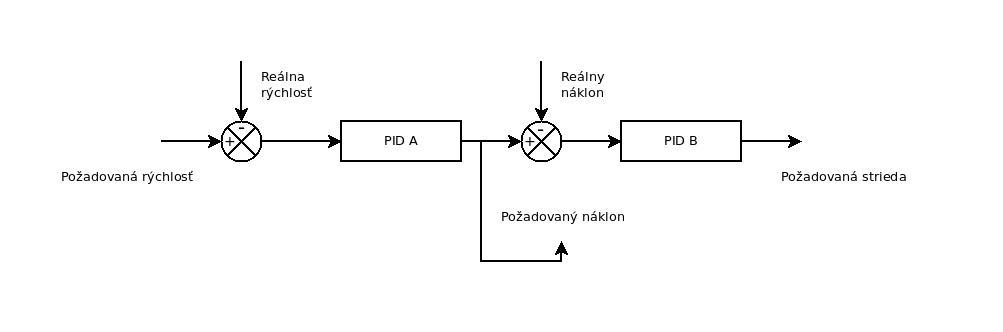
\includegraphics[width=16cm]{PID_robota}
\caption{Schematické zapojenie PID regulátorov}
\label{fig:RS}
\end{figure}

\underline{\textbf{PID A}}:
Vstupom do PID A je požadovaná rýchlosť robota, tá je následne odčítaná od reálnej rýchlosti nameranej pomocou enkodérov a spracovaná PID regulátorom. Pri riadení robota môžeme špecifikovať požadovanú rýchlosť a na výstupe PID A bude požadovaný uhol náklonu. Týmto spôsobom zabezpečíme  dosiahnutie požadovanej rýchlosti aj to, že robot sa bude pohybovať konštantnou rýchlosťou. Výhodnou vlastnosťou PID A je, že požadovaný uhol náklonu nebude počas celej doby riadenia konštantný pre danú rýchlosť, ale bude dynamicky prispôsobovaný aktuálnym podmienkam. 

Ak by to tak nebolo a robot by sa snažil pri pohybe udržiavať konštantný uhol náklonu, musel by neustále zrýhľovať lebo len tak by mohol zabrániť pádu. Tento stav by trval až pokiaľ by motory dosiahli maximálnu rýchlosť a neboli naďalej schopné zabezpečiť konštantné zrýchľovanie robota. Po tomto bode by nasledoval pád.

\underline{\textbf{PID B}}:
Výstupom PID B je ako už bolo skôr spomenuté strieda signálu vstupujúceho do H-mostíka. V prípade nami použitého mostíka platí priama úmera medzi striedou vstupného signálu a napätím do motorov. Nedá sa ale povedať, že by závislosť medzi striedou a výstupným napätím bola lineárna. V skutočnosti pre efektívne napätie na výstupe mostíka platí vzťah \eqref{eq:RMSSquare}, v ktorom $\delta$ je z intervalu $<0;1>$ a predstavuje striedu vstupného signálu. Závislosť výstupného napätia a striedy je zobrazená na \figurename~\ref{fig:strieda_napatie}. V našom prípade ale nejde o závažný nedostatok, ktorý by výrazným spôsobom ovplyvňoval výsledky regulácie.
\begin{equation}
U_{EF} = U_{MAX}\sqrt{\delta}
\label{eq:RMSSquare}
\end{equation}
\begin{figure}[h!]
\centering
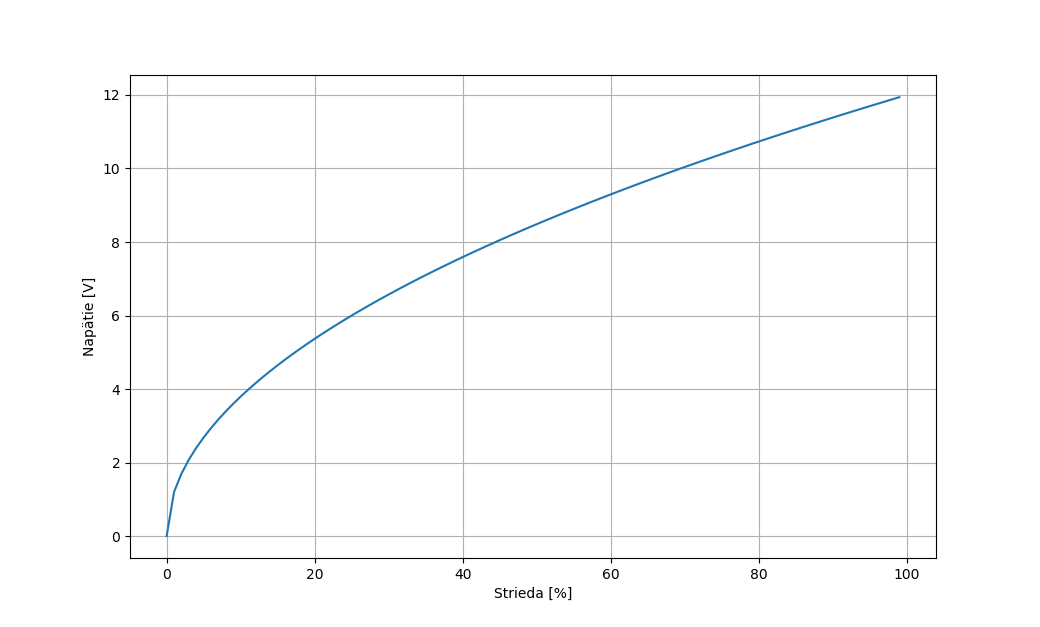
\includegraphics[width=14cm]{strieda_napatie}
\caption{Znázornenie závislosti medzi striedou a napätím}
\label{fig:strieda_napatie}
\end{figure}
Ladenie \ac{RS} prebiehalo po častiach. Ako prvý sme naladili PID B, pričom využitá bola Zieger-Nicholsova metóda, nasledovaná jemným manuálnym doladením parametrov. Pri ladení bol na vstup privedený nulový vstupný signál, reprezentujúci požiadavku na nulový uhol náklonu. Výsledkom tohto ladenia bol robot schopný balansovať vo vzpriamenej polohe a taktiež odolať aj silnejším pokusom o jeho prevrhnutie. Ako nedostatkom sa ale javilo to, že robot nebol nijakým spôsobom penalizovaný za pohyb, a tak trvalo aj niekoľko sekúnd kým sa po postrčení opäť dostal do ustáleného stavu (stav charakterizovaný minimálnou osciláciou okolo osi natočenia a minimálnou rýchlosťou pohybu).

Po naladení PID B bol ladený PID A, pričom sme na vstup RS opäť priviedli nulovú hodnotu - teda požiadavku na nulovú rýchlosť. Keďže pri prevádzke bude práve tento stav s nulovou požiadavkou najčastejší, pri ladení PID A sa kládol silný dôraz na správanie systému pri návrate do ustáleného stavu. PID A bol naladený obdobným spôsobom ako PID B. Výsledkom bol \ac{RS} schopný zabezpečiť minimálnu uhlovú výchylku robota pri minimálnej rýchlosti pohybu.

Keďže pri realizáciu PID bola použitá forma popísaná v \ref{eq:compPID}, bolo ešte potrebné určiť konštantu $T_f$ podľa vzťahu \ref{eq:TFconst}. Pri zisťovaní oscilačnej frekvencie robota pri pohybe sme na presné zmeranie krátkych periód oscilácií použili kamerový záznam pohybu robota. Pri známej frekvencii snímkovania, ktorá bola v našom prípade 60 \ac{FPS} (frames per second), je spočítaním snímok a ich vynásobením periódou snímkovania možné presne odmerať aj krátke časové okamihy. Zavedenie konštanty $T_f$ zlepšilo vlastnosti \ac{RS} robota.

Takto naladené PID regulátory pracujú v zapojení do kaskády, pričom PID B pracuje s periódou 10ms a PID A s periódou 50ms. Tento čas je dostatočný na to, aby bol robot schopný rýchlo reagovať na podnety a dostatočne dlhý na to aby sme mohli získať a spracovať dáta zo senzorov. Dôvodom relatívne dlhej periódy PIDu B je princíp fungovania enkodéra, z ktorého by sme pri výrazne kratšej perióde meraní neboli schopní vypočítať rýchlosť s dostatočnou presnosťou.   

\section{Implementácia riadiaceho systému}
Implementácia \ac{RS} robota bola realizovaná v jazyku C++, pričom sme využili objektovo orientovaný spôsob programovania. V praxi to znamená, že jednotlivé funkčné celky robota sú reprezentované v dátových štruktúrach nazývaných objekty. Každý objekt predstavuje inštanciu triedy, v ktorej sú definované jeho vlastnosti a metódy - teda jeho štruktúra. Prostredníctvom týchto vlastností a metód objekt vykonáva v rámci funkčného celku určité funkcie. Výhodou tohto postupu je, že takto napísaný kód je znovu použiteľný aj v iných projektoch a v prípade potreby jednoducho rozšíriteľný o dodatočnú funkcionalitu. Zapuzdrenie jednotlivých funkčných celkov taktiež pomáha udržiavať kód prehľadný.

Príkladom triedy v nami použitom kóde je napríklad trieda \textit{PID}. V tejto triede sú definované metódy, ktoré by mal byť každý objekt triedy PID schopný realizovať. V našom prípade ide o metódy pre nastavenie a úpravu parametrov P, I, D a metódu pre vypočítanie výstupe PIDu vzhľadom na určitý vstup. Vytvorenie tejto triedy nám umožnilo reprezentovať PID A a PID B ako inštancie tejto triedy. 

Pri triede PID je treba poznamenať, že priame použitie \ref{eq:compPID} na vypočítanie výstupu by nebolo možné, keďže v nami predstavenej forme sa jedná o spojitý regulátor. Mikroprocesor je ale digitálne zariadenie, ktoré nie je schopné priamo realizovať spojitú funkciu, ani prijímať spojité dáta (ktoré by väčšina nami použitých senzorov ani nebola schopná poskytnúť). Je preto potrebné vyjadriť \ref{eq:compPID} aj vo spojitej forme. Výstup PID pre vzorku číslo $i$ je teda:
\begin{equation}
y_i = Pe_i + I\sum_{k=0}^{i}{e_k}\Delta t + D\Delta e_i 
\end{equation}
pričom $e_i$ je rozdiel požadovaného uhla a skutočného uhla, pre vzorku $i$, $\Delta t$ je čas medzi jednotlivými vzorkami a $\Delta e_i$ je možné vyjadriť ako:
\begin{equation}
\Delta e_i = \dfrac{T_f\Delta e_{i-1} + (e_i - E_{i-1})}{\Delta t + T_f}
\end{equation}


\listingname~\ref{lst:PIDsample} predstavuje ukážku jednej nami implementovanej metódy triedy PID. Jej výstup predstavuje výstup daného PID regulátora.  


\begin{inlinecode}[label={lst:PIDsample},caption={Príklad jednej z metód triedy PID}]{c++}
float PID::giveOutput(float input, float target, float dt, float constrainI){
    float output  = 0;
    float Perror = target-input;
    error_integral += Perror;
    if(constrainI){
        error_integral = constrain(error_integral,-constrainI,constrainI);
    };
    error_derivative = (Tf*error_derivative + (Perror - old_error))/(dt + Tf);       //implements filtering constant Tf
    output = P*(Perror)+I*(error_integral)*dt+D*error_derivative;

    old_error = Perror;
    return output;
}
\end{inlinecode}

Celý nami vytvorený kód pracuje po úvodnej inicializácii premenných a vytvorení objektov na princípe kontrolnej slučky, t.j. skupiny príkazov, ktoré sa periodicky opakujú. V našom prípade sme túto slučku navrhli tak, aby prebehla raz za každých 10 ms. V tejto riadiacej slučke načítavame nové údaje zo senzorov, spracovávame ich prostredníctvom \ac{RS} a na vstup H-mostíka privádzame výsledný signál \ac{PWM}. Celý proces je znázornený v diagrame \figurename~\ref{fig:simpleFlowchart}.

V \figurename~\ref{fig:simpleFlowchart} nie sú znázornené spracovania prerušení, v ktorých sa spracúvajú údaje z enkodérov, použitých na monitorovanie aktuálnej rýchlosti robota. Výstup zo samotných enkodérov prichádza do mikropočítača po štyroch dátových linkách (dve pre každý enkodér), vo forme impulzov vzájomne oneskorených o čas $t_e$. Výstup z dvoch kanálov enkodéra je zobrazený na \figurename~\ref{fig:enkoder}. Na jedinú otáčku kolesa pripadá $N$ takto vzájomne posunutých impulzov (pre jeden kanál). Spočítaním týchto impulzov za čas  $t_S$ vieme určiť uhlovú rýchlosť kolesa $\omega$ a z nej následne odvodiť celkovú rýchlosť pohybu robota. Smer pohybu určíme podľa poradia detekcie impulzov. Vzorec pre výpočet rýchlosti pohybu robota je teda možné vyjadriť ako:
\begin{equation}
\begin{gathered}
\Delta\phi_w = \dfrac{2\pi}{N}k \qquad [rad] \\
\omega = \dfrac{\Delta\phi_w}{t_S} \qquad [rad.s^{-1}]\\
v = \omega r \qquad[m.s^{-1}]
\end{gathered}
\label{eq:speedEq}
\end{equation}


kde $\Delta\phi_w$ predstavuje zmenu uhla natočenia kolesa $k$ predstavuje počet detegovaných impulzov z jednej linky za čas $t_S$ a $r$ polomer kolesa robota.

Následne je ešte potrebné zredukovať šum prítomný v takto nameraných dátach. V našom prípade sme postupovali pomocou metódy ukladania nameraných hodnôt z enkodérov do FIFO buffera a ich vyhodnotením podľa vzťahu: 
\begin{equation}
k = \dfrac {k_n - k_{n-j}}{j}
\end{equation}
kde $j+1$ bol maximálny počet uložených hodnôt.

Z tohto vzťahu sme získali hodnotu $k$, z ktorej je možné dosadením do vzťahu \ref{eq:speedEq} získať priemernú rýchlosť robota medzi meraniami $n-j$ a $n$. My sme pracovali s hodnotou $j=9$ (10 uložených vzoriek), pričom sme nové hodnoty získané z odometrických meraní vkladali do buffera každých 25ms. Keďže reakcie motora sú ale relatívne pomalé, údaje o rýchlosti robota boli v PIDe A vyhodnocované každých 50ms.  

Pri filtrovaní a fúzii dát nameraných z akcelerometra a gyroskopu používame komplementárny filter v tvare:
\begin{equation}
\alpha_n = c(\alpha_{n-1}+\Delta\alpha_{n}) + (1-c)(\beta_n)
\end{equation}
kde:

$c$ = konštanta komplementárneho filtra

$\alpha_n$ = výstup z komplementárneho filtra pre meranie $n$

$\alpha_{n-1}$ = výstup z komplementárneho filtra pre meranie $n-1$

$\Delta\alpha_{n}$ = zmena uhla medzi meraniami $n$ a $n-1$ získaná z gyroskopu 

$\beta_n$ = uhol z akcelerometra pre meranie $n$


Podrobná schéma zobrazujúca celkovú činnosť \ac{RS} robota je na \figurename~\ref{fig:podrobna_schema}. Znázorňuje RS robota aj spôsob spracovania dát na jeho vstupoch.
\begin{figure}[!b]
\centering
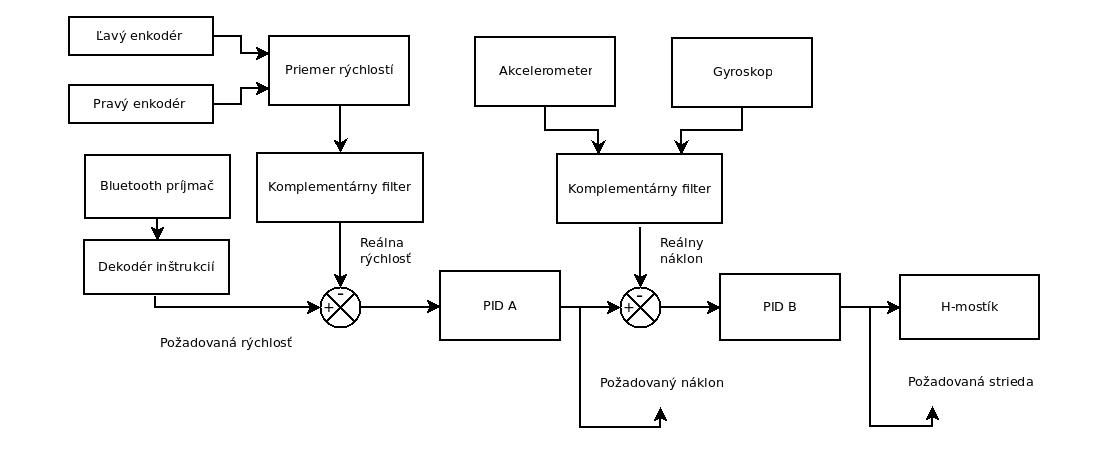
\includegraphics[width=15cm]{comp_RS_diagram}
\caption{Podrobná schéma RS robota}
\label{fig:podrobna_schema}
\end{figure}

Zaujímavosťou je, že pri fúzii dát z gyroskopu a akcelerometra sa ukázalo ako výhodné v komplementárnom filtri s postupom času potláčať vplyv merania z akcelerometra až po dosiahnutie určitej konečnej hodnoty. Dôvodom je, že pri spustení potrebuje robot chvíľu na to, aby presne zistil svoj uhol natočenia, tento môže presne získať len z akcelerometra. Po zorientovaní a správnom nastavení polohy je výhodné potlačiť vplyv akcelerometra, čím sa zamedzí vplyvu náhodných otrasov a silných postrčení na presnosť merania uhla. Merania z akcelerometera sú totiž pri náhlych zmenách polohy omnoho menej presné ako tie z gyroskopu.

\section{Ovládanie pohybu robota}
Použitím komunikačného rozhrania využívajúceho technológiu Bluetooth sme zabezpečili jednoduchú a dostatočne rýchlu komunikáciu medzi robotom a ovládačom, prostredníctvom ktorého je operátor schopný jednoducho zadávať robotovi príkazy. Následne ale bolo potrebné zabezpečiť, aby sa tieto príkazy spoľahlivo premietali do riadenia pohybov robota. Taktiež bolo potrebné zabezpečiť, aby robot nebol závislý od príkazov operátora a dokázal balansovať na mieste aj bez prítomnosti riadiaceho signálu.

Riadiaci signál prichádzajúci z ovládača prenáša riadiace príkazy vo forme jednotlivých bajtov, pričom prvý bajt slúži ako jedinečný identifikátor príkazu. Takýmto spôsobom sme zabezpečili jednoduché odlíšenie až 256 jedinečných príkazov, ktoré robot môže od ovládača prijať. V prípade príkazu prenášajúceho pohybové povely bude tento prvý jedinečný identifikátor nasledovaný dvoma bajtami dát, ktoré obsahujú preškálované hodnoty z 10-bitového prevodníka ADC v ovládači, napojeného na X-ovú a Y-ovú os analógového joypadu.  

Dosiahnutie plynulého riadenia rýchlosti po prijatí riadiaceho bajtu bolo jednoduché. Hodnota prijatá z X-ovej osi joypadu sa preškáluje z rozsahu 0-100 na $-v_d$ až $v_d$. Túto hodnotu po preškálovaní ozn. $v_s$ a použitá je ako vstup do PID A. Po praktickom testovaní rôznych hodnôt $v_d$ sme vo finálnej verzii robota použili hodnotu $v_d = 7$. V praxi hodnota $v_d$ predstavuje max. rýchlosť pohybu robota v $rad.s^{-1}$.

Praktické testy ďalej ukázali, že pred vložením vypočítanej rýchlosti $v_s$ na vstup PID A je vhodné použiť komplementárny filter, ktorý spomalí rýchlosť nárastu $v_s$. Týmto postupom sme docielili plynulejšie zrýchlenie a spomalenie robota, čo v konečnom dôsledku prispelo k celkovému zlepšeniu stability robota.

Ako problematické sa v praxi ale ukázalo riadenie smeru robota. Pri prvých pokusoch sme prijatú hodnotu z Y-osi joypadu preškálovali a filtrovali spôsobom analogickým ako pri riadení rýchlosti a takto získanú hodnotu $o_s$ sme používali pri riadení motorov. V prípade ľavotočivej zatáčky tak bola k hodnote požadovanej striedy pravého motora pripočítaná hodnota $o_s$ a od striedy ľavého odpočítaná (opačne pre pravotočivú zatáčku). Tento systém spoľahlivo pracoval pri rozbehnutom robotovi, ale ukázal sa ako nedostatočný pri pokusoch otáčať nehybného robota.

Problémom pri otáčaní nehybného robota bol fakt, že v skutočnosti nie je možné dosiahnuť balansovanie robota bez rýchlych zmien striedy vstupujúcej do H-mostíka. Tieto zmeny striedy sú natoľko rýchle, že v praxi sa prejavia len jemným chvením robota, ale pri snahe upravovať striedu o hodnotu $o_s$ dôjde len k trhaným pohybom robota na mieste. Tento nedostatok sa nám nepodarilo odstrániť ani zmenou parametrov komplementárneho filtra ani zmenami $o_s$.

Ako uspokojivé riešenie sa nakoniec ukázalo riadenie zatáčania za jazdy pomocou $o_s$ a riadenie otáčania na mieste priamym zavedením predefinovanej striedy na oba motory, podľa požadovaného smeru otáčania a pri dodržaní maximálnej dovolenej rýchlosti robota, pri ktorej je ešte možné otočku vykonať. Pri tomto spôsobe otáčania ostáva strieda motorov po určitý krátky čas stabilná a dostatočne veľká na to, aby spôsobila otočenie robota na mieste bez výrazného narušenia jeho stability. 

\section{Podporné metódy riadenia}
Pri testovaní RS sme zvažovali aj niektoré ďalšie podporné, metódy riadenia správania sa robota. Tieto sme nepovažovali za natoľko kritické, aby ich bolo nutné uplatniť ako hlavnú časť \ac{RS}, ale keďže ich implementácia nebola náročná, rozhodli sme sa ich zahrnúť do celkového dizajnu robota.

Jedným z menej závažných problémov pri nami navrhnutom robotovi bola jeho neschopnosť zotrvať na jednom mieste pri balansovaní s nulovou požiadavkou na rýchlosť. Aj keď tento problém sme do značnej miery eliminovali regulovaním požadovanej rýchlosti, robot aj tak nebol schopný nijakým spôsobom určovať svoju pozíciu v priestore. Následkom toho bolo, že po postrčení sa robot niekedy nevrátil presne do miesta, v ktorom pôvodne balansoval. Tento problém sa prejavoval aj pri dlhodobom balansovaní bez externých stimulov. Kvôli náhodným osciláciám pri balansovaní a nerovnakou charakteristikou motorov (ktorú sa nepodarilo celkom odstrániť ani zavedením kalibračných konštánt) sa robot pomaly pohyboval priestorom v okolí bodu, kde začal balansovať.  

Prvou z týchto podporných metód bolo teda zaradenie dodatočného, tretieho PID C regulátora pred hlavnú RS \figurename~\ref{fig:thridPID} .Tento regulátor má na svojom vstupe celkovú prejdenú vzdialenosť robota za celú dobu jeho prevádzky, získanú z enkodérov. Jeho výstupom je požadovaná rýchlosť, pri ktorej dodržaní sa robot dostane späť na miesto, v ktorom začal balansovať. 

Tento tretí PID C v praxi fungoval výborne, ale ani s jeho použitím sa však nepodarilo úplne odstrániť problém s nerovnomerným pohybom motorov. Tento spôsob riadenia je taktiež nepoužiteľný pri ovládanom pohybe, pri ktorom by zaradenie PID C spôsobovalo nestabilitu systému. Aj z tohoto dôvodu sme sa rozhodli, že PID C bude pri ovládaní robota permanentne odpojený a zaradiť do RS sa bude dať len manuálne pokynom z ovládača a to len v režime balansovania na mieste. 

\begin{figure}[h]
\centering
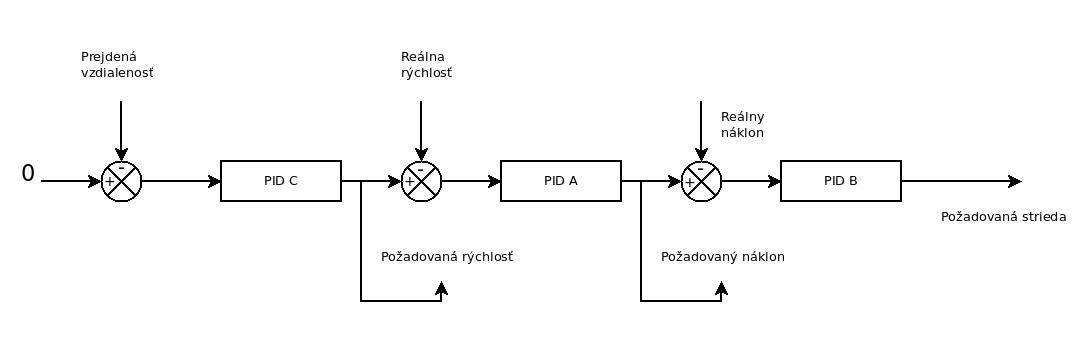
\includegraphics[width=16cm]{additionalPid}
\caption{Upravený RS}
\label{fig:thridPID}
\end{figure}


Ďalšou metódou, ktorá mala pôvodne byť súčasťou hlavnej časti RS robota, bolo meranie elektrického prúdu vstupujúceho do H-mostíka. Myšlienkou bolo navrhnúť a skonštruovať elektrický obvod, ktorý by s použitím tohto merania a dát z mikropočítača bol schopný generovať požadovaný prúd pre motory. 

Výhodou tohto postupu by bolo presnejšie riadenie motorov. Dôvodem je, že točivý moment motorov je úmerný prúdu, ktorý nimi tečie - nie napätiu samotnému. Pri balansovaní na mieste, kde sú potrebné rýchle a presné reakcie motorov, by sme teda teoreticky mohli priamym riadením momentu motorov dosiahnuť menšie oscilácie pri pohybe.

Meranie prúdu bolo zabezpečené rezistorom s malým odporom \figurename~\ref{fig:currentSensor} zaradeným do série s H-mostíkom. Meraním úbytku napätia na tomto odpore sme pri známej hodnote odporu $R$ schopní vypočítať prúd tečúci odporom do H-mostíka. Toto zapojenie bolo realizované na nami navrhnutom shielde, v praxi sa ale ukázalo ako nepoužiteľné.

Dôvodom bol fakt, že vstupom do H-mostíka neboli plynule sa meniaci prúd a napätie, ale PWM napájanie. Z tohto dôvodu nami odmeraný prúd nezávisel na reálnom prúde vstupujúcom do motorov, ale na tom, ktorú časť PWM sa podarilo ovzorkovať. Tento nedostatok sme sa pokúsili kompenzovať kondenzátorom paralelne pripojeným k rezistoru voči nulovému potenciálu. Výsledky ale neboli uspokojivé ani v tomto zapojení. Meranie prúdu sme teda po úvahe vyradili a nebrali ďalej do úvahy.



 
  

 
